\documentclass[../Book.Stress_regulation.tex]{subfiles}
\graphicspath{{\subfix{../images/}}}
\begin{document}

\label{Ex:SunSalutation}
\begin{figure}[htb!]
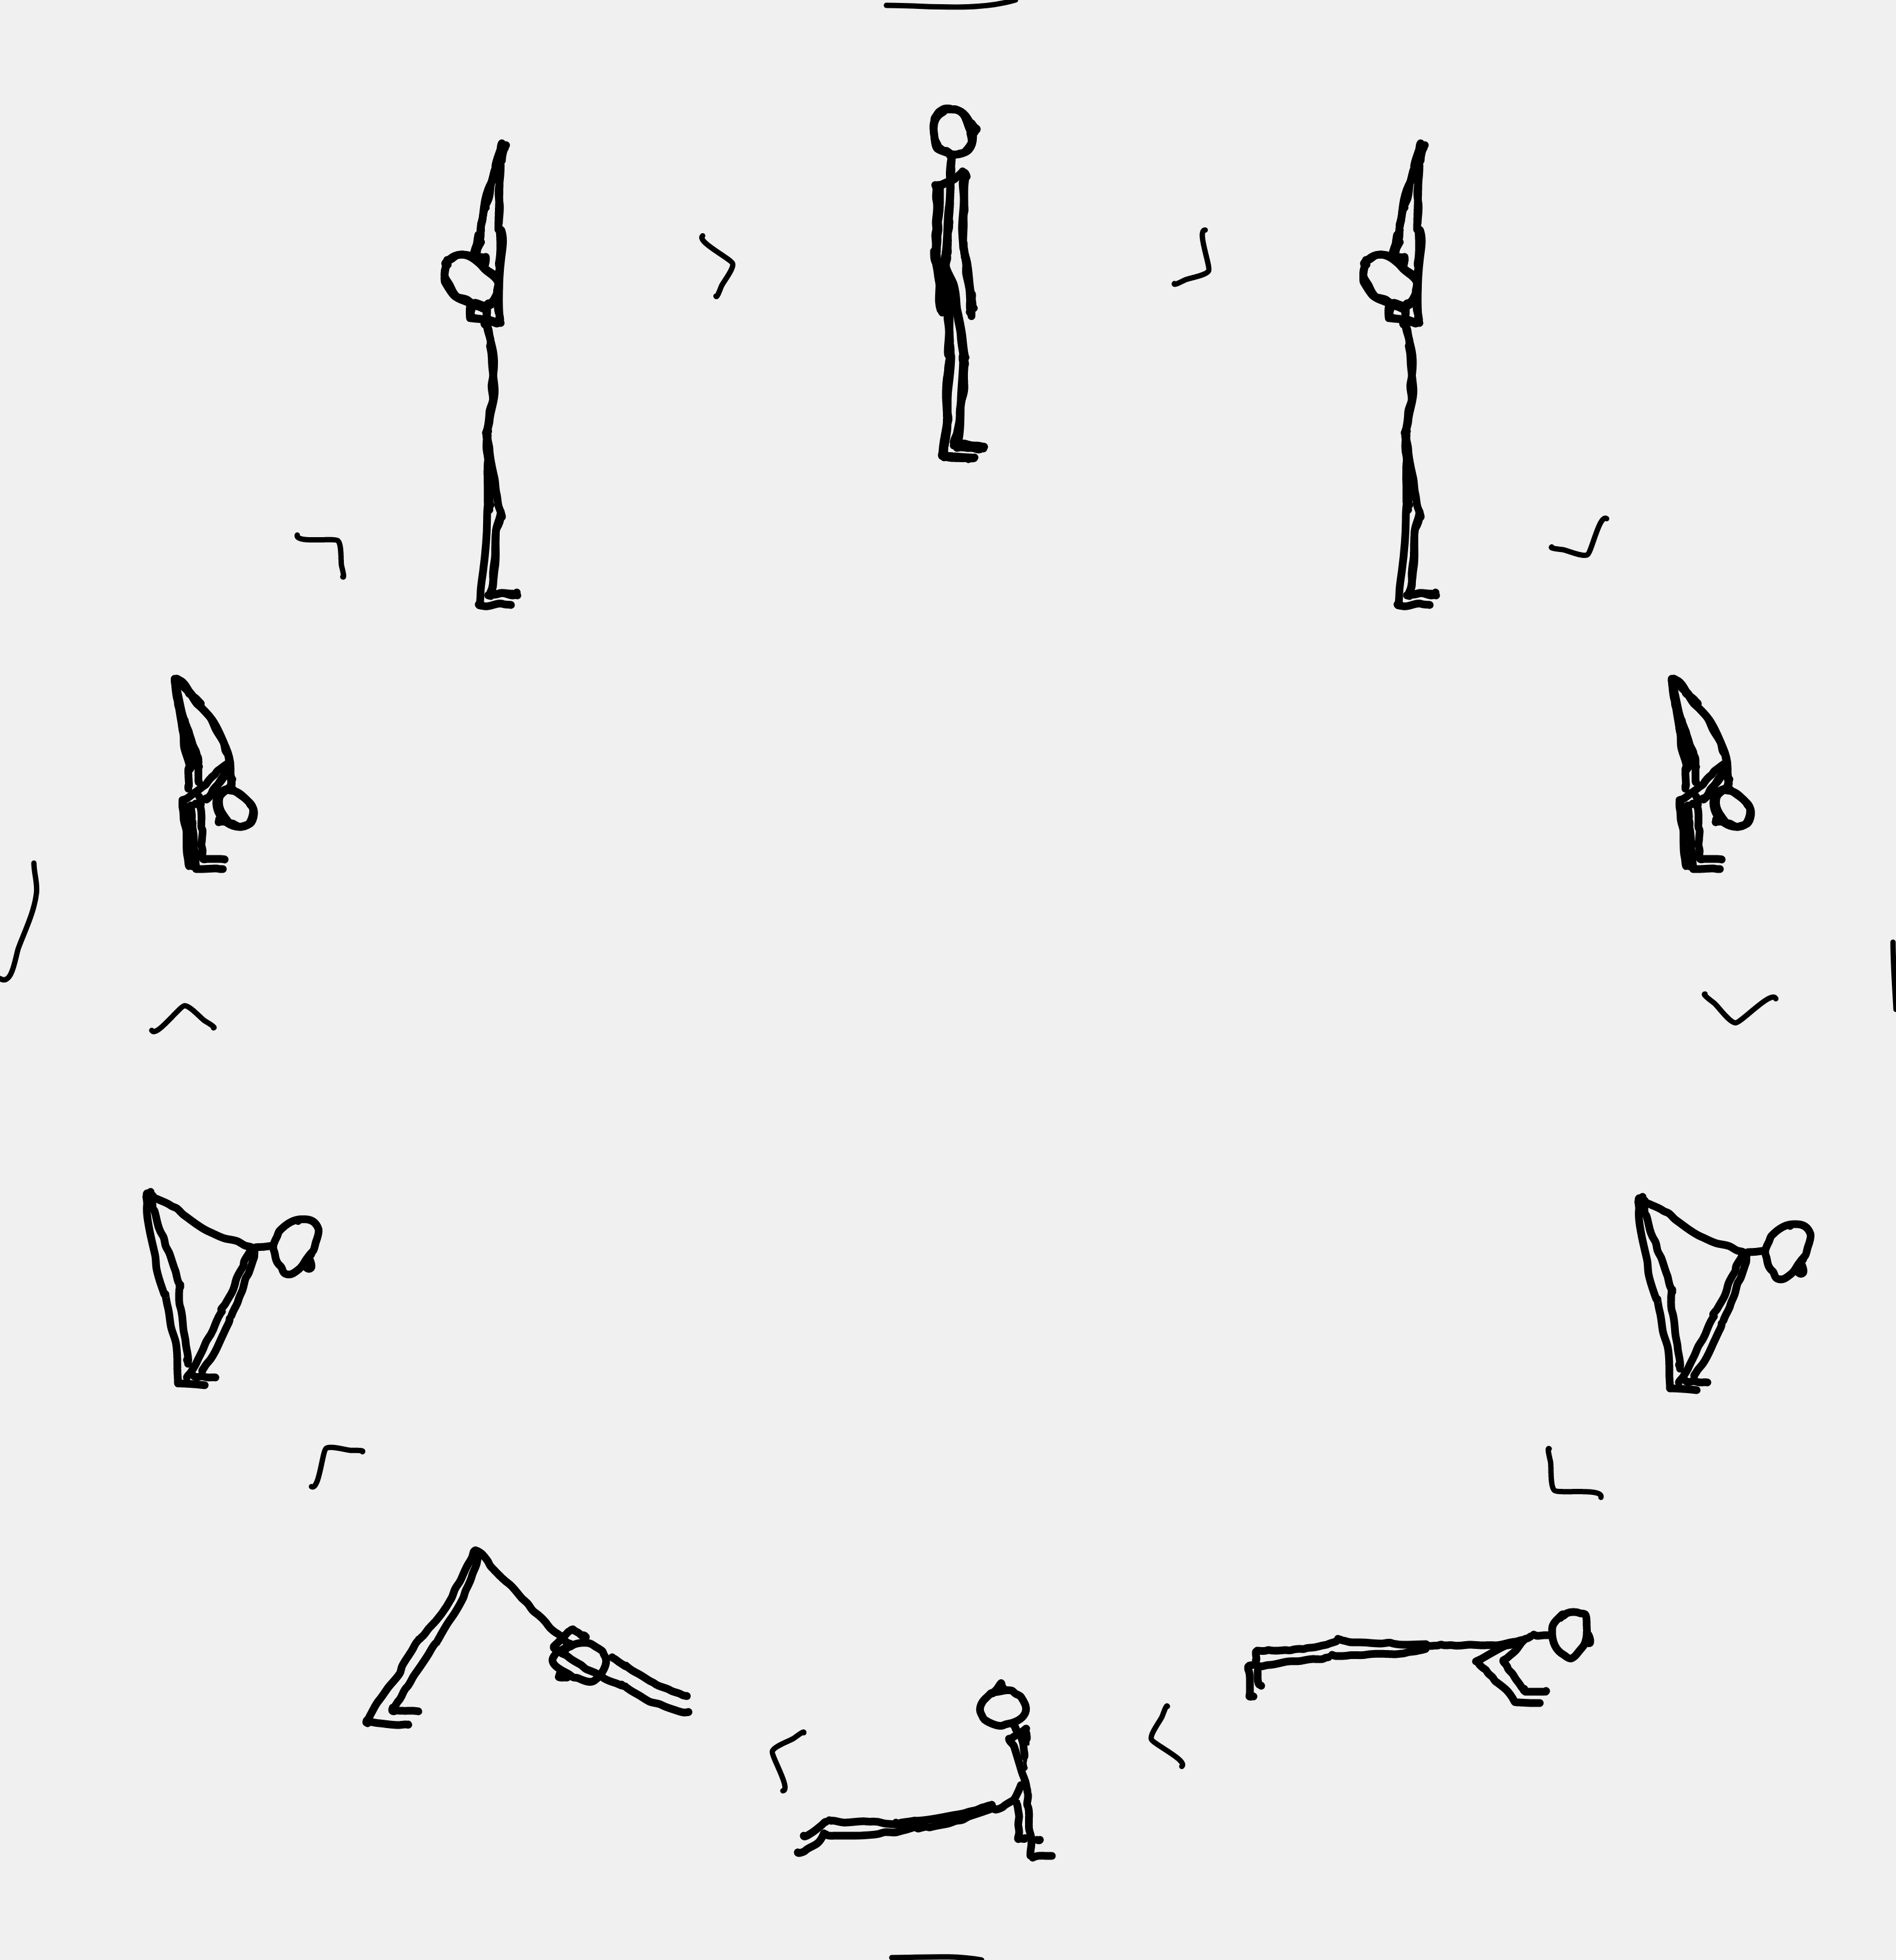
\includegraphics[width=13cm]{SunSalute}
\caption{Sun salutation --- Surya Namaskar}
\end{figure}

%------------------------------------------------------------
%------------------------------------------------------------

The Sun Salutation\index{sun salutation} increases your physical strength, flexibility, your inner balance and your mental clarity.
Practiced first thing in the morning, it gets you instantaneously awake and active.
Practiced in the evening, it helps free up blocked energies.
The Sun Salutation stimulates all internal organs, stretches and twists the spinal cord, all the limbs and all muscle groups.
\end{document}